\documentclass[11pt,a4paper]{article}
\usepackage[margin=2.4cm]{geometry}
\usepackage[T1]{fontenc}
\usepackage[utf8]{inputenc}
\usepackage{lmodern}
\usepackage{amsmath,amssymb}
\usepackage{booktabs}
\usepackage{graphicx}
\usepackage{caption}
\usepackage{longtable}
\usepackage{enumitem}
\usepackage{xcolor}
\usepackage{url}
\usepackage[hidelinks]{hyperref}
\usepackage{microtype}
\graphicspath{{figures/}}
\setlength{\parskip}{4pt}
\captionsetup{font=small,labelfont=bf}

\newcommand{\code}[1]{\texttt{#1}}
\newcommand{\HV}{\mathrm{HV}}
\newcommand{\IGD}{\mathrm{IGD}}

\title{\textbf{Reproducing LLM-NAS and Extending It to Hardware-Aware Search\\ for Small Language Models}\\[4pt]
\large A reproducibility study and framework report}
\author{Siyabonga Mjali\thanks{Implementation and experiments were carried out with AI-assisted tooling (Claude Code). All numbers in this report are generated by the code in the accompanying repository and can be regenerated from the archived run logs.}}
\date{10 October 2026}

\begin{document}
\maketitle

\begin{abstract}
This report documents (i) an independent reproduction of \emph{LLM-NAS: LLM-Driven Hardware-Aware Neural Architecture Search} (Zhu, Zhang \& Huang, 2025) on HW-NAS-Bench, and (ii) an extension that blends the LLM-NAS search engine with \emph{LiteTransformerSearch} (Javaheripi et al., 2022) and the \emph{Small Language Models} survey (Lu et al., 2024) in order to search for hardware-efficient decoder-only transformers. We built a single, configuration-driven Python framework in which every large-language-model (LLM) call is logged and replayable, every run is keyed by a hash of its configuration, and every paper table maps to one command. Data-alignment checks confirm that our benchmark tables are the ones the paper used (11 of 12 reported Table-2 points are recovered exactly), while uncovering one point that does not exist in the benchmark and a benchmark artefact (4{,}699 missing Edge-TPU latencies stored as $-1$) that silently corrupts hypervolume unless handled. Running the method with GPT-4.1 and with a local Qwen2.5-7B model, we find that under any reasonable hypervolume convention the LLM operator does \emph{not} outperform cheap non-LLM baselines inside the paper's own complexity niches: random sampling within niches reaches $\HV=0.991\pm0.001$ on CIFAR-10/Edge GPU against $0.964$ (GPT-4.1, one seed) and $0.888$ (Qwen). The niche partitioning itself, the paper's central mechanism, is confirmed as the component that matters. In the transformer extension (36 runs, 6 methods, 2 device models, 3 seeds), the same pattern holds under a sharper metric we introduce, \emph{latency overhead at matched quality}: random sampling within decoder-parameter niches achieves $+5.2\%\pm0.8$ against $+8.4\%\pm4.8$ for LLM-NAS with Qwen ($p=0.04$), while removing niches is worst ($+10.1\%$, 88\% coverage). Seeding the LLM with published design insights had no measurable effect ($p=0.94$). We discuss why hypervolume saturates in these spaces, list every unspecified hyper-parameter and the choice made, and propose the experiments that would settle the open question of whether the LLM's benefit depends on model capability.
\end{abstract}

\tableofcontents
\newpage

%=====================================================================
\section{Introduction}
Hardware-aware neural architecture search (HW-NAS) seeks architectures that trade off task performance against on-device cost (latency, memory, energy). Supernet-based methods achieve strong results but cost GPU-days per dataset. LLM-NAS \cite{llmnas} proposes replacing both the supernet and the evolutionary operator with a large language model that (a) is confined to \emph{complexity niches} to counteract its tendency to propose familiar designs (\emph{exploration bias}), (b) co-evolves a textual \emph{knowledge base} of design rules alongside the architectures, and (c) scores candidates with a training-free zero-cost (ZC) predictor. The paper reports near-perfect Pareto fronts (hypervolume $\HV\approx0.99$) on HW-NAS-Bench at a cost of 120 API calls.

This work had three goals, pursued in sequence:
\begin{enumerate}[nosep]
  \item Build an \emph{organised, re-runnable} reproduction of LLM-NAS suitable for a PhD workflow: one command per table or figure, exact replay without API access, and an explicit record of every assumption.
  \item Run the reproduction with the paper's LLM (GPT-4.1) and with an open 7B model (Qwen2.5-7B) and compare against the ablations the paper reports.
  \item Transfer the framework to a new domain, hardware-efficient small language models (SLMs), by blending it with two further papers, and test whether the LLM operator's benefit carries over.
\end{enumerate}
Sections~\ref{sec:background}--\ref{sec:cnnresults} cover goals 1--2; Sections~\ref{sec:blend}--\ref{sec:slmresults} cover goal 3; Section~\ref{sec:discussion} synthesises what was discovered; Section~\ref{sec:future} lists next steps. A glossary of all technical terms and formulas is given in Appendix~\ref{sec:glossary}.

%=====================================================================
\section{Background: the three papers}\label{sec:background}

\paragraph{LLM-NAS \cite{llmnas}.} The search space is the NAS-Bench-201 cell: six edges, each carrying one of five operators (\code{none}, \code{skip\_connect}, \code{nor\_conv\_1x1}, \code{nor\_conv\_3x3}, \code{avg\_pool\_3x3}), giving $5^6=15{,}625$ architectures. HW-NAS-Bench \cite{hwnasbench} supplies measured latency for each on six devices. The method (Algorithm~1 of the paper) partitions the space into six disjoint niches by the number of $3{\times}3$ convolutions (Table~1 of the paper), keeps a Pareto archive per niche, and in each of 10 generations asks the LLM first to update a knowledge base of ``use/avoid \ldots because \ldots'' rules and then to propose children by crossover or mutation. Fitness is the HW-NAS-Bench latency plus the output of an XGBoost regressor over the 13 zero-cost proxies of NAS-Bench-Suite-Zero \cite{nbsz}. Quality is reported as hypervolume (HV) and inverted generational distance (IGD) against the true Pareto front.

\paragraph{LiteTransformerSearch (LTS) \cite{lts}.} LTS observes that for autoregressive transformers, the \emph{decoder (non-embedding) parameter count} ranks fully-trained models by perplexity with Spearman correlation 0.97--0.99, irrespective of topology, whereas latency and memory vary up to $2.8\times$ and $5.5\times$ at fixed parameter count. It therefore searches a heterogeneous per-layer GPT-2/Transformer-XL space with an evolutionary algorithm, using parameter count as a free quality proxy and measuring latency and memory directly on the target device.

\paragraph{SLM survey \cite{slmsurvey}.} Lu et al.\ catalogue 70 open decoder-only models of 100M--5B parameters, finding that by 2024 the typical SLM uses grouped-query attention, a gated (SwiGLU) feed-forward block with intermediate ratio 2--8, RMSNorm and a large vocabulary. Their on-device measurements (Jetson Orin NX, three smartphones, \code{llama.cpp}, 4-bit weights) show that prefill is compute-bound and shape-sensitive, decode is memory-bound and roughly linear in parameter bytes, the KV cache dominates memory at long context, and vocabulary size inflates the compute buffer. They also note that latency clusters into 0.1--1B, 1--2B and 2--3B bands.

The three fit together: LTS says quality is ``free'' given size and the real problem is \emph{shape}; the survey explains \emph{which} shapes are cheap and why; LLM-NAS supplies a search engine designed for problems whose structure is known qualitatively, and its niching idea maps directly onto the survey's size bands.

%=====================================================================
\section{Reproduction methodology}\label{sec:method}

\subsection{Framework design}
The implementation is a single Python package (\code{llmnas}, $\approx$3{,}700 lines including tests) with the following properties, all motivated by the need to regenerate thesis numbers years later:
\begin{itemize}[nosep]
  \item \textbf{One configuration system.} \code{configs/base.yaml} holds every default, each tagged \code{[paper]} (stated in the paper) or \code{[assumed]} (our choice). Experiment files define a grid (datasets $\times$ devices $\times$ seeds) and named variants as overrides.
  \item \textbf{Content-addressed runs.} A run lives at \path{results/runs/<variant>-<hash8>/<dataset>/<device>/seed<k>/}, where the hash covers the effective configuration (excluding fields that cannot change results, such as the replay flag and the client timeout). A finished run is never recomputed; interrupted grids resume; changing any setting creates a new directory rather than overwriting.
  \item \textbf{Replayable LLM calls.} Every prompt, response, token count and wall time is appended to \code{llm\_calls.jsonl}. Running with \code{llm.mode=replay} feeds the saved responses back and must reproduce the run bit-for-bit (a mismatch counter must read zero). This was verified for both the CNN and the transformer searches.
  \item \textbf{Provenance.} Each run records the git commit (and a dirty flag) that produced it.
  \item \textbf{Pluggable LLM backends.} Any OpenAI-compatible endpoint (GPT-4.1, OpenRouter, Ollama), Anthropic Claude, or an offline mock used only for tests.
  \item \textbf{Tests.} 44 pytest cases run on synthetic data without the 2\,GB download, including end-to-end searches with the mock backend and exact-replay checks.
\end{itemize}

\subsection{Data}
Three public sources were merged into one tidy table per dataset (15{,}625 rows each):
HW-NAS-Bench v1.0 (latency on Edge GPU, Raspberry Pi 4, Edge TPU, Pixel 3, Eyeriss, FPGA);
NAS-Bench-Suite-Zero \code{zc\_nasbench201.json} (13 ZC proxies and validation accuracy);
and NATS-Bench \cite{nats} (200-epoch \emph{test} accuracy, which is what the paper's Table~2 reports, e.g.\ the 94.37\% CIFAR-10 optimum).
NASLib encodes architectures with a different operator order and edge permutation from the NB201 string; the mapping (\code{[skip,none,conv3,conv1,pool]}, edge permutation $[0,1,3,2,4,5]$) was verified by matching validation accuracies on all 15{,}625 architectures.

\subsection{Predictor, metrics and search}
\textbf{Predictor.} An XGBoost regressor (500 trees, depth 6) on the 13 ZC proxies, trained on 1{,}000 random architectures labelled with NB201 \emph{validation} accuracy, predicts for the whole space once so the search does $O(1)$ lookups. The Synflow ablation maps the raw Synflow score to the accuracy scale by isotonic regression (ranking unchanged).

\textbf{Metrics.} Both objectives are minimised internally as (latency, $-$accuracy). Objectives are min--max normalised by the ideal and nadir points of the true front $P^\ast$, the reference point is $r=(1.1,1.1)$, and we report $\HV(S)/\HV(P^\ast)$ and IGD (formulas in Appendix~\ref{sec:glossary}). The paper gives neither its normalisation nor its reference point; because it reports $\HV\le1$ and ``near-perfect'' values, a ratio is the most plausible reading.

\textbf{Search.} Algorithm~1 of the paper with switches for every ablation: \code{partitioning} (six niches vs.\ the whole space), \code{operator} (\code{llm} | \code{random} = the paper's PEA ablation | \code{random\_sample}), \code{knowledge\_base} on/off, and \code{predictor.kind} (\code{zc\_ensemble} | \code{synflow} | \code{oracle}). Un-partitioned variants receive the same evaluation budget (30 initial samples, 240 proposals) as partitioned ones. Prompts follow Appendix~E of the paper verbatim where text is given; the architecture legend and parent tables fill the paper's placeholders.

\subsection{Unspecified details and the choices made}\label{sec:assumed}
Table~\ref{tab:assumed} lists what the paper leaves open. These are the first things to vary in a sensitivity study.
\begin{table}[h]\centering\small
\caption{Choices not specified by LLM-NAS (all exposed in \code{configs/base.yaml}).}\label{tab:assumed}
\begin{tabular}{p{4.6cm}p{4.0cm}p{6.2cm}}
\toprule
Item & Choice & Rationale \\
\midrule
Initial population per niche & 5 random architectures & Algorithm~1 samples but gives no size \\
Children per Stage-2 call & 4 & $6\times10\times4=240$ proposals over 120 calls \\
Parents shown per prompt & $\le6$ (half newest, rest random) & Fig.~4 shows both ``last cycle'' and ``random from archive'' \\
Crossover probability $p_c$ & each child slot assigned crossover w.p.\ 0.5 & reconciles Sec.~4.1 ($p_c{=}0.5$) with App.~E (LLM decides) \\
Knowledge-base scope & one per niche & Stage-1 prompt contains the niche definition \\
Invalid / duplicate / out-of-niche proposals & discarded, no retry, counted & keeps the 120-call budget fixed \\
\code{latency\_limit} in prompt & omitted & never given a value \\
Temperature & 0.7 & not stated (Claude backends ignore it) \\
Predictor training set & 1{,}000 archs, validation labels & ``trained on a sample''; avoids test leakage \\
Accuracy for HV/IGD & NB201 200-epoch test accuracy & Table~2 reports the 94.37\% test optimum \\
Discovered set $S$ & final front of Algorithm~1 (selected by predicted accuracy), re-scored with true accuracy & Algorithm~1 returns $P_{\text{final}}$ \\
HV/IGD normalisation & true-front min--max, $r=(1.1,1.1)$, HV as ratio & paper reports $\HV\le1$ \\
Seeds & 3 & paper reports $\pm$ without a count \\
\bottomrule
\end{tabular}
\end{table}

%=====================================================================
\section{Reproduction results}\label{sec:cnnresults}

\subsection{Data-alignment checks}
\begin{itemize}[nosep]
  \item Best test accuracies match NB201 exactly: 94.37 / 73.51 / 47.31 (CIFAR-10 / CIFAR-100 / ImageNet16-120).
  \item \textbf{11 of the 12} LLM-NAS points in the paper's Table~2 exist in the benchmark with matching accuracy \emph{and} latency. The exception is Edge GPU ``94.37\% @ 4.35\,ms'': the 94.37\% architecture \code{(3,3,3,1,3,2)} runs at 6.81\,ms on Edge GPU, and no architecture has that pair. The identical row is printed for PRP-NAS-BA, suggesting a transcription error.
  \item All five example rows in the paper's Figure~2 match CIFAR-100/Edge GPU to within rounding, which also confirms the 6-tuple encoding used in the paper.
  \item \textbf{Benchmark artefact.} HW-NAS-Bench stores $-1$ as the Edge TPU latency of 4{,}699 architectures (30\%); the other five devices are complete. Treated as real values, these produce fake zero-cost points on the ``true'' front and collapse Edge TPU HV to $\approx0.2$ for every method; treated as unmeasured (our choice), Edge TPU behaves like the other devices ($\HV\approx0.92$). The paper does not say how it handled this.
  \item The ZC-ensemble predictor reaches Spearman $0.960\pm0.001$, $0.964\pm0.001$ and $0.957\pm0.002$ against test accuracy on the three datasets, above the paper's $\approx0.90$; Synflow alone reaches 0.75--0.78. Niche sizes are 729 / 3{,}367 / 6{,}144 / 3{,}840 / 1{,}280 / 265 architectures for S0--S5.
\end{itemize}

\subsection{Main comparison on CIFAR-10 / Edge GPU}
Table~\ref{tab:cnn} and Figure~\ref{fig:cnnfronts} compare the full method under two LLMs with the non-LLM baselines on the paper's headline setting. GPT-4.1 was run once (120 calls, 8.6\,min, 160{,}319 input and 66{,}747 output tokens, $\approx\$0.85$ at list price); Qwen2.5-7B (4-bit, Ollama, 8K context) ran once on an RTX~3050~Ti laptop GPU (153\,min). The baselines were run with three seeds.

\begin{table}[h]\centering\footnotesize
\caption{CIFAR-10, Edge GPU. HV$\uparrow$ as a fraction of the true front's HV; IGD$\downarrow$ in normalised units. ``Usable'' = proposals that were valid, inside their niche and not duplicates; ``Eval.'' = distinct architectures evaluated (both are means over seeds for the controls). Paper values from its Table~3, which also reports FairNAS 0.892\,/\,0.073, PRP-NAS 0.843\,/\,0.116 and LLMatic 0.191\,/\,0.542 (HV\,/\,IGD).}\label{tab:cnn}
\setlength{\tabcolsep}{4pt}
\begin{tabular}{llccccc}
\toprule
Method & LLM & Seeds & HV & IGD & Usable & Eval. \\
\midrule
LLM-NAS (paper) & GPT-4.1 & ? & 0.997 & 0.006 & -- & -- \\
LLM-NAS (ours) & GPT-4.1 & 1 & 0.964 & 0.063 & 99/240 (41\%) & 129 \\
LLM-NAS (ours) & Qwen2.5-7B & 1 & 0.888 & 0.088 & 95/240 (40\%) & 125 \\
PEA: niches, random operators & -- & 3 & $0.989\pm0.004$ & $0.038\pm0.008$ & 155/240 (65\%) & 185 \\
Random sampling in niches & -- & 3 & $0.991\pm0.001$ & $0.052\pm0.012$ & 239/240 (100\%) & 269 \\
\bottomrule
\end{tabular}
\end{table}

\begin{figure}[h]\centering
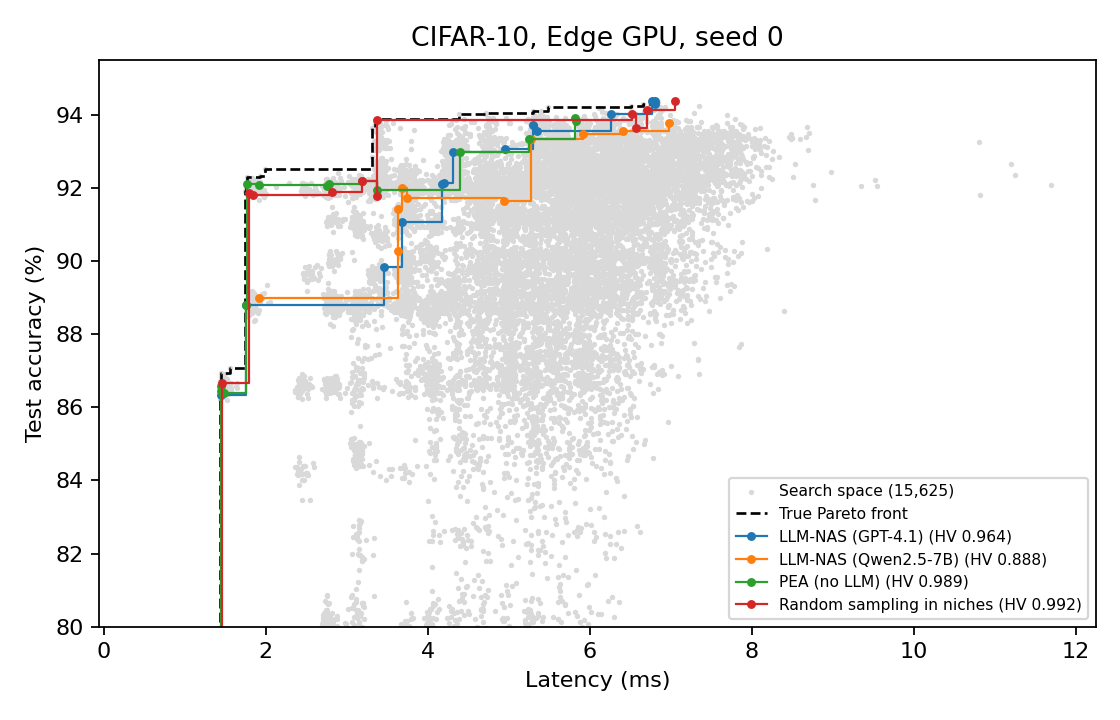
\includegraphics[width=0.8\textwidth]{cnn_fronts_edgegpu.png}
\caption{Final fronts on CIFAR-10 / Edge GPU (seed 0) against the true Pareto front. Both LLM variants miss the fastest region of the front; GPT-4.1 does recover the 94.37\% optimum.}\label{fig:cnnfronts}
\end{figure}

Three observations follow. First, GPT-4.1 improves on Qwen (0.964 vs.\ 0.888), and its knowledge base contains sensible rules (e.g.\ for niche S3: ``maintain exactly two \code{nor\_conv\_3x3} \ldots assign them to later or output-related edges''), but it still discards 59\% of its own proposals, 107 of them as duplicates of architectures it had already been shown. Second, both LLM variants are dominated by random proposals \emph{inside the same niches}, which reach $\HV\approx0.99$ with no API calls. Third, the HV trajectories (GPT-4.1: $0.883\!\to\!0.964$ in a single jump at generation~7; random: $0.883\!\to\!0.990$ by generation~5) show that the initial 30 random samples already achieve $\HV=0.883$ under this normalisation, so the metric leaves only $\approx0.11$ of head-room for any search procedure.

\subsection{Ablation on CIFAR-100 (paper's Table 5)}
The paper reports that removing the LLM operator (PEA) drops average HV on CIFAR-100 from 0.978 to $0.843\pm0.075$. With our normalisation, PEA alone achieves $0.946\pm0.031$ averaged over the six devices (three seeds each), and uniform random sampling within niches $0.931\pm0.047$ (Figure~\ref{fig:abl}). The gap between our PEA and the paper's PEA ($\approx0.10$) is larger than the gap the paper attributes to the LLM, which means the HV convention, not the operator, is the dominant unknown. We also noticed that the paper's Table-5 average HV for the full model (0.978) is not the mean of its six Table-3 CIFAR-100 values (0.982), although the IGD average does match.

\begin{figure}[h]\centering
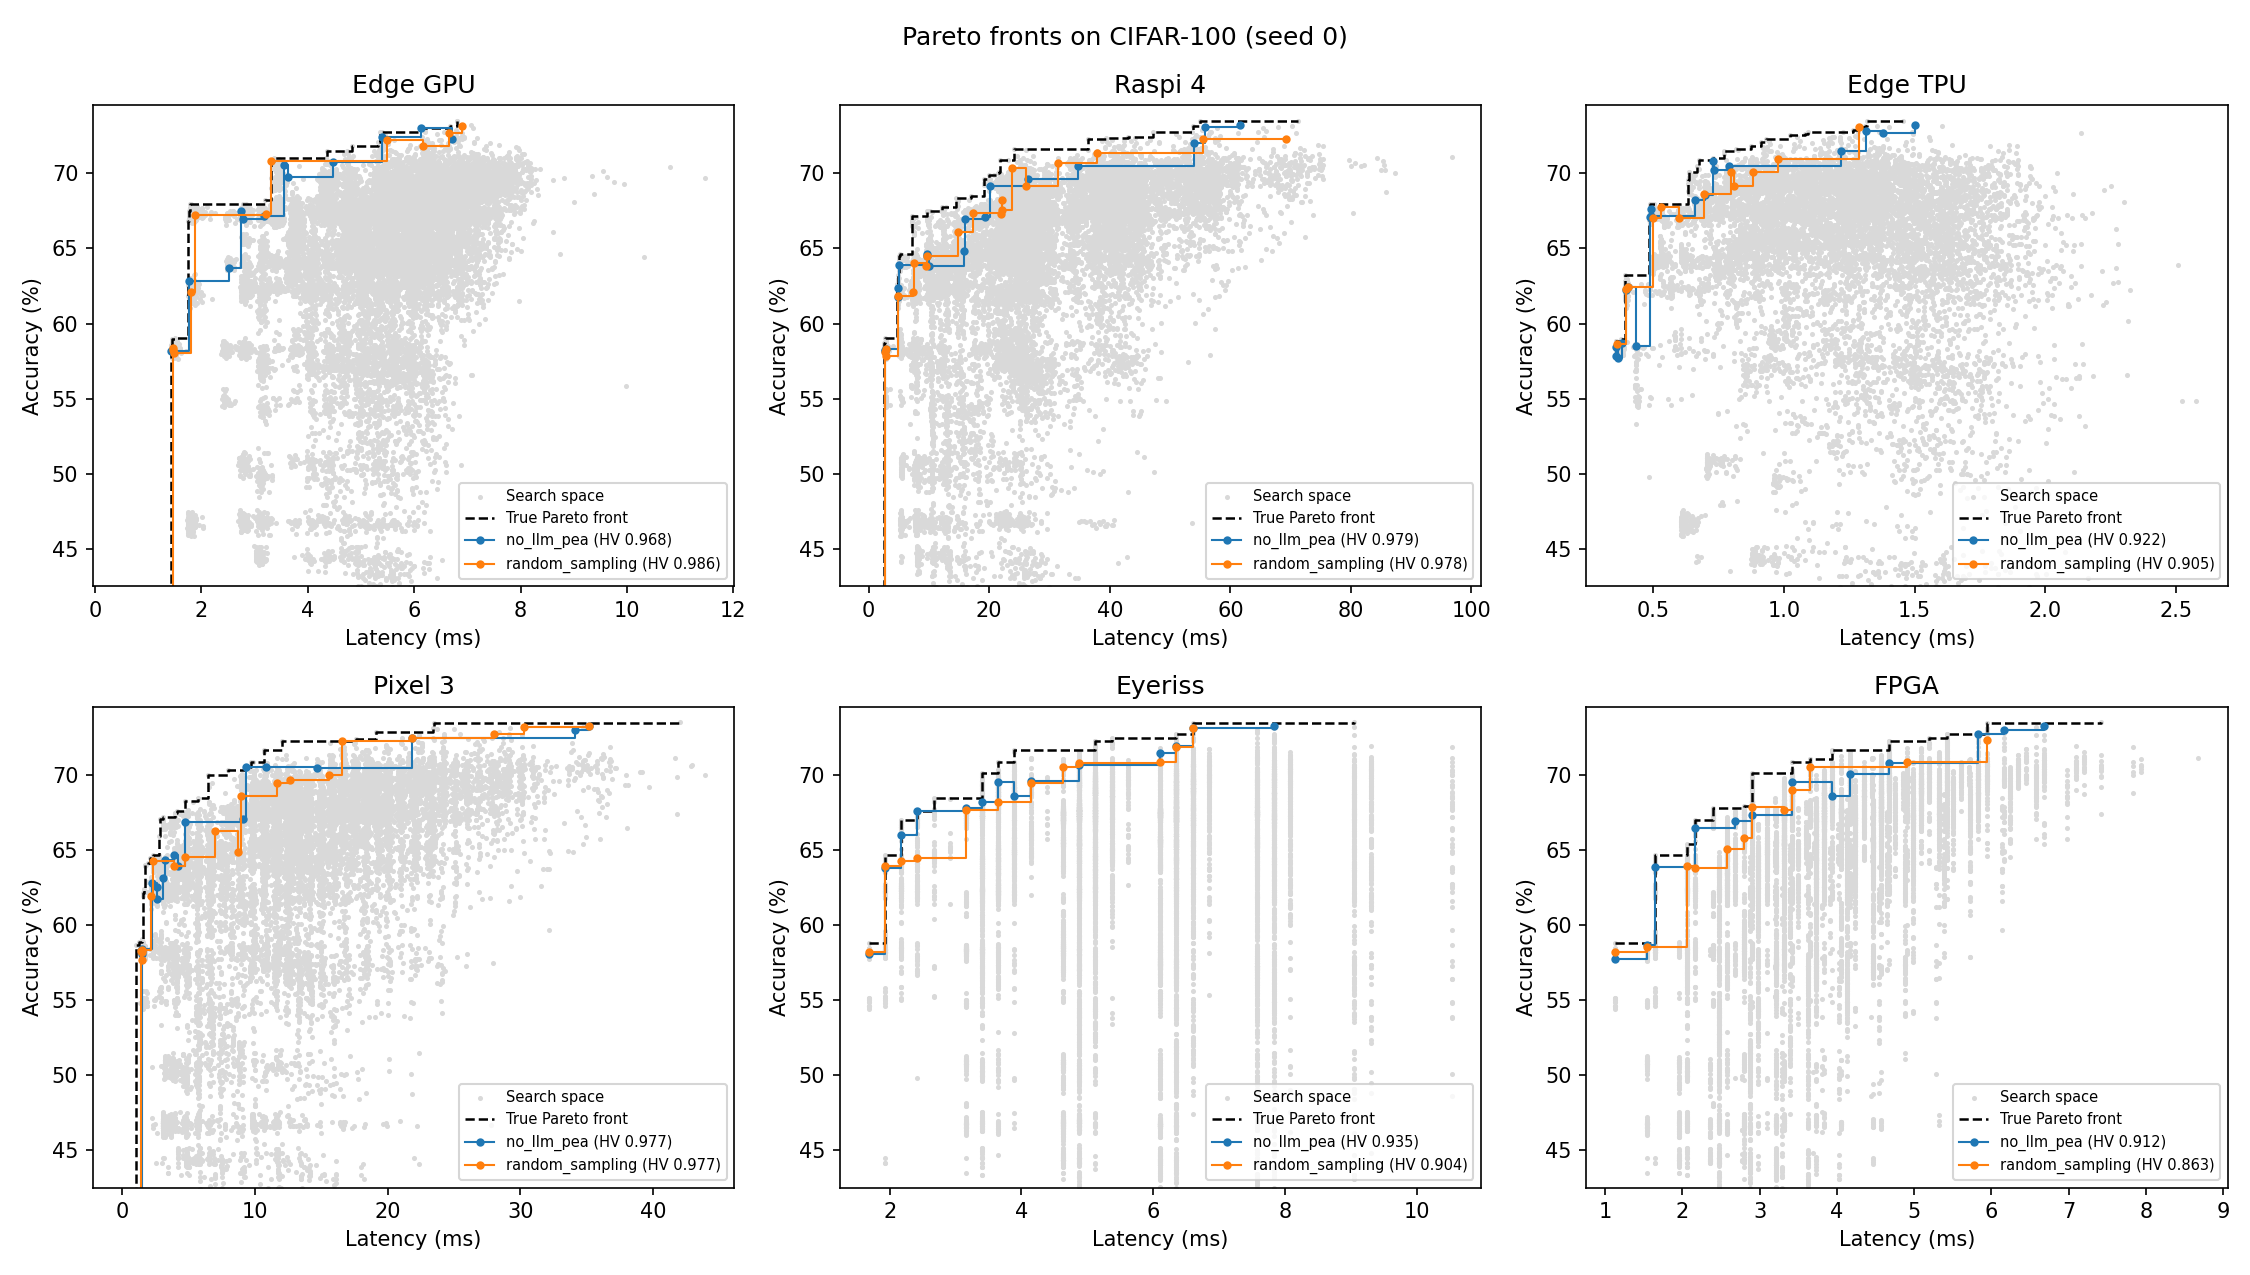
\includegraphics[width=\textwidth]{fronts_cifar100.png}
\caption{Non-LLM fronts on CIFAR-100 for all six devices (seed 0). Edge TPU is shown after excluding unmeasured ($-1$) latencies.}\label{fig:abl}
\end{figure}

%=====================================================================
\section{Extension: hardware-aware search for small language models}\label{sec:blend}

\subsection{Design}
We kept the LLM-NAS engine unchanged and replaced the search space, the quality proxy and the hardware model:
\begin{itemize}[nosep]
  \item \textbf{Search spaces.} \code{slm}: a homogeneous decoder with $n_{\text{layer}}\in[8,40]$, $d_{\text{model}}\in[512,3072]$ (step 128), gated FFN with $d_{\text{inner}}/d_{\text{model}}\in[2,8]$, head dimension $\in\{64,128\}$, $n_{\text{kv}}\in\{1,2,4,8,n_{\text{head}}\}$, vocabulary 32K, tied embeddings (ranges from the survey's Table~1 and Figure~2). \code{lts\_gpt2}: LTS's heterogeneous per-layer GPT-2 space ($n_{\text{layer}}\in[2,16]$, $d_{\text{model}}\in[128,1024]$, $d_{\text{inner}}\in[256,4096]$, $n_{\text{head}}\in\{2,4,8\}$).
  \item \textbf{Niches} are disjoint bands of decoder parameters ($<$250M, 250--500M, 0.5--1B, 1--2B, 2--3B, $\ge$3B), the transformer analogue of Table~1 of LLM-NAS and aligned with the survey's latency bands. Figure~\ref{fig:niches} is the analogue of LLM-NAS's Figure~3: each band occupies a distinct latency range, and each spans roughly $2\times$ in latency, so there is room to optimise shape within a niche.
  \item \textbf{Quality} is LTS's decoder-parameter count, shown to the LLM as the Kaplan scaling-law loss $L(N)=(N_c/N)^{0.076}$, which is monotone and therefore ranks identically.
  \item \textbf{Hardware} follows the survey's decomposition: prefill time $\approx\max(F/\Theta,\,B/\beta)$ for FLOPs $F$, weight bytes $B$, effective throughput $\Theta$ and bandwidth $\beta$, plus a per-layer overhead; decode time $\approx$ (bytes read per token)$/\beta$ plus overhead; memory = quantised weights + KV cache (2{,}048 context) + compute buffer ($512\times V\times4$ bytes). Device profiles for the survey's Jetson Orin NX and Snapdragon 8 Gen 1 phone were fitted by eye to the survey's plots; profiles for the local RTX~3050~Ti and CPU can be \emph{calibrated} by least squares against measurements.
  \item \textbf{Measurement} (LTS-style): each candidate is instantiated in PyTorch with random weights; prefill and KV-cached decode are timed and peak memory recorded; results are cached per device. Calibrating on 20 random GPT-2-space models on the local CPU gave Spearman 0.977 and 4.8\% mean absolute error between modelled and measured latency; an in-loop measured search evaluated 78 architectures in 7.5 minutes.
  \item \textbf{Prior knowledge.} The \code{survey\_kb} variant starts the knowledge base from the survey's ``Insights'' boxes and LTS's shape finding, e.g.\ ``use fewer, wider layers when prefill latency matters, because prefill is compute-bound and every extra layer adds fixed overhead''.
  \item \textbf{Reference models.} Eleven real SLMs (SmolLM-135M/360M/1.7B, Qwen2.5-0.5B/1.5B/3B, TinyLlama-1.1B, Llama-3.2-1B/3B, Pythia-1.4B, Phi-2) are encoded from their public configurations; our parameter formula reproduces their official sizes to within 0.4\%.
\end{itemize}

\begin{figure}[h]\centering
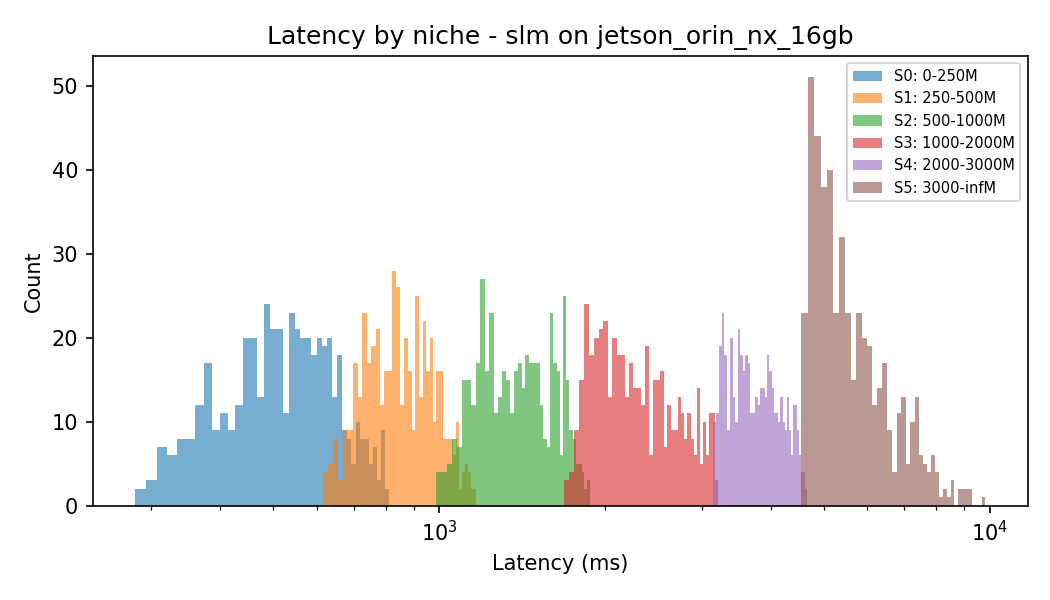
\includegraphics[width=0.72\textwidth]{niches_slm_jetson_orin_nx_16gb.png}
\caption{Latency distribution of random architectures in each decoder-parameter niche (Jetson Orin NX cost model). The clustering mirrors LLM-NAS's Figure~3 and the survey's observed latency bands.}\label{fig:niches}
\end{figure}

\subsection{Variants and evaluation}
Six variants share the same budget (30 initial samples plus 240 proposals): \code{llmnas} (unchanged engine), \code{llmnas\_survey\_kb} (survey prior), \code{no\_partitioning} (LLM without niches), \code{lts\_search} (LTS's own algorithm: global Pareto-front evolution, mutation probability 0.3, plus crossover), \code{no\_llm\_pea} (niches + random evolution), and \code{random\_sampling}. The experiment grid is 2 device models $\times$ 3 seeds; the LLM was Qwen2.5-7B (16K context, 8{,}192-token replies), 120 calls per search, $\approx$2.7--3.3\,h per search on the laptop GPU (36 runs, $\approx$33\,h of wall time).

Because no exhaustive ground truth exists, HV and IGD are computed against the \emph{pooled reference front} of all feasible architectures evaluated by any run for that (space, device). As anticipated, HV saturates (0.966--0.992 for every variant) because every niche-based method covers all sizes. We therefore introduced a sharper primary metric, \textbf{latency overhead at matched quality}: for 40 log-spaced decoder-parameter levels $N$ across the pooled front, let $t^\ast(N)$ be the lowest latency of any model with $\ge N$ decoder parameters found by \emph{any} run and $t_m(N)$ the same for run $m$; the overhead is the geometric mean of $t_m(N)/t^\ast(N)$ minus one over the levels the run reaches, and \emph{coverage} is the fraction of levels reached (Appendix~\ref{sec:glossary}). This reads directly as ``how much slower is this method's best model at a given quality''.

%=====================================================================
\section{Extension results}\label{sec:slmresults}

\begin{table}[h]\centering\small
\caption{\code{slm} space, mean $\pm$ s.d.\ over 6 runs (3 seeds $\times$ 2 device models). Overhead = latency overhead at matched quality (lower is better). HV$_2$ = hypervolume on (quality, latency) against the pooled front.}\label{tab:slm}
\begin{tabular}{lcccccc}
\toprule
Variant & Overhead & Jetson & Snapdragon & Coverage & Usable & HV$_2$ \\
\midrule
Random sampling in niches & $\mathbf{+5.2\%\pm0.8}$ & $+5.0\%$ & $+5.3\%$ & 96\% & 100\% & 0.99 \\
LTS search & $+6.1\%\pm2.3$ & $+5.8\%$ & $+6.4\%$ & 92\% & 94\% & 0.98 \\
PEA (niches, random operators) & $+6.3\%\pm2.9$ & $+6.5\%$ & $+6.1\%$ & 98\% & 98\% & 0.99 \\
LLM-NAS + survey prior (Qwen) & $+7.8\%\pm3.4$ & $+9.1\%$ & $+6.5\%$ & 95\% & 50\% & 0.98 \\
LLM-NAS (Qwen) & $+8.4\%\pm4.8$ & $+6.7\%$ & $+10.0\%$ & 95\% & 49\% & 0.98 \\
LLM-NAS, no niches (Qwen) & $+10.1\%\pm2.6$ & $+8.7\%$ & $+11.5\%$ & \textbf{88\%} & 50\% & 0.97 \\
\bottomrule
\end{tabular}
\end{table}

\begin{table}[h]\centering\small
\caption{Latency overhead per niche (mean over seeds and devices). S0 is the hardest band for every method.}\label{tab:niche}
\begin{tabular}{lcccccc}
\toprule
Variant & S0 $<$250M & S1 & S2 & S3 & S4 & S5 $\ge$3B \\
\midrule
Random sampling & 8.7\% & 4.4\% & 2.5\% & 2.2\% & 1.4\% & 2.8\% \\
LTS search & 11.3\% & 2.2\% & 2.7\% & 1.4\% & 2.1\% & 3.1\% \\
PEA & 10.4\% & 4.4\% & 4.3\% & 3.8\% & 2.2\% & 2.7\% \\
LLM-NAS + survey prior & 10.6\% & 6.6\% & 9.2\% & 5.4\% & 3.4\% & 3.5\% \\
LLM-NAS & 12.5\% & 6.1\% & 8.2\% & 5.3\% & 4.1\% & 3.4\% \\
No niches & 13.3\% & 7.0\% & 9.1\% & 6.8\% & 9.1\% & 6.3\% \\
\bottomrule
\end{tabular}
\end{table}

Mann--Whitney $U$ tests on the six runs per variant give: random sampling vs.\ LLM-NAS $p=0.041$; random sampling vs.\ LLM-NAS+prior $p=0.093$; PEA vs.\ LLM-NAS $p=0.31$; LLM-NAS vs.\ LLM-NAS+prior $p=0.94$; LLM-NAS vs.\ no niches $p=0.13$. Figure~\ref{fig:slmfronts} shows the (quality, latency) and (quality, memory) fronts with the real SLMs overlaid; Figure~\ref{fig:slmconv} the convergence of HV.

\begin{figure}[h]\centering
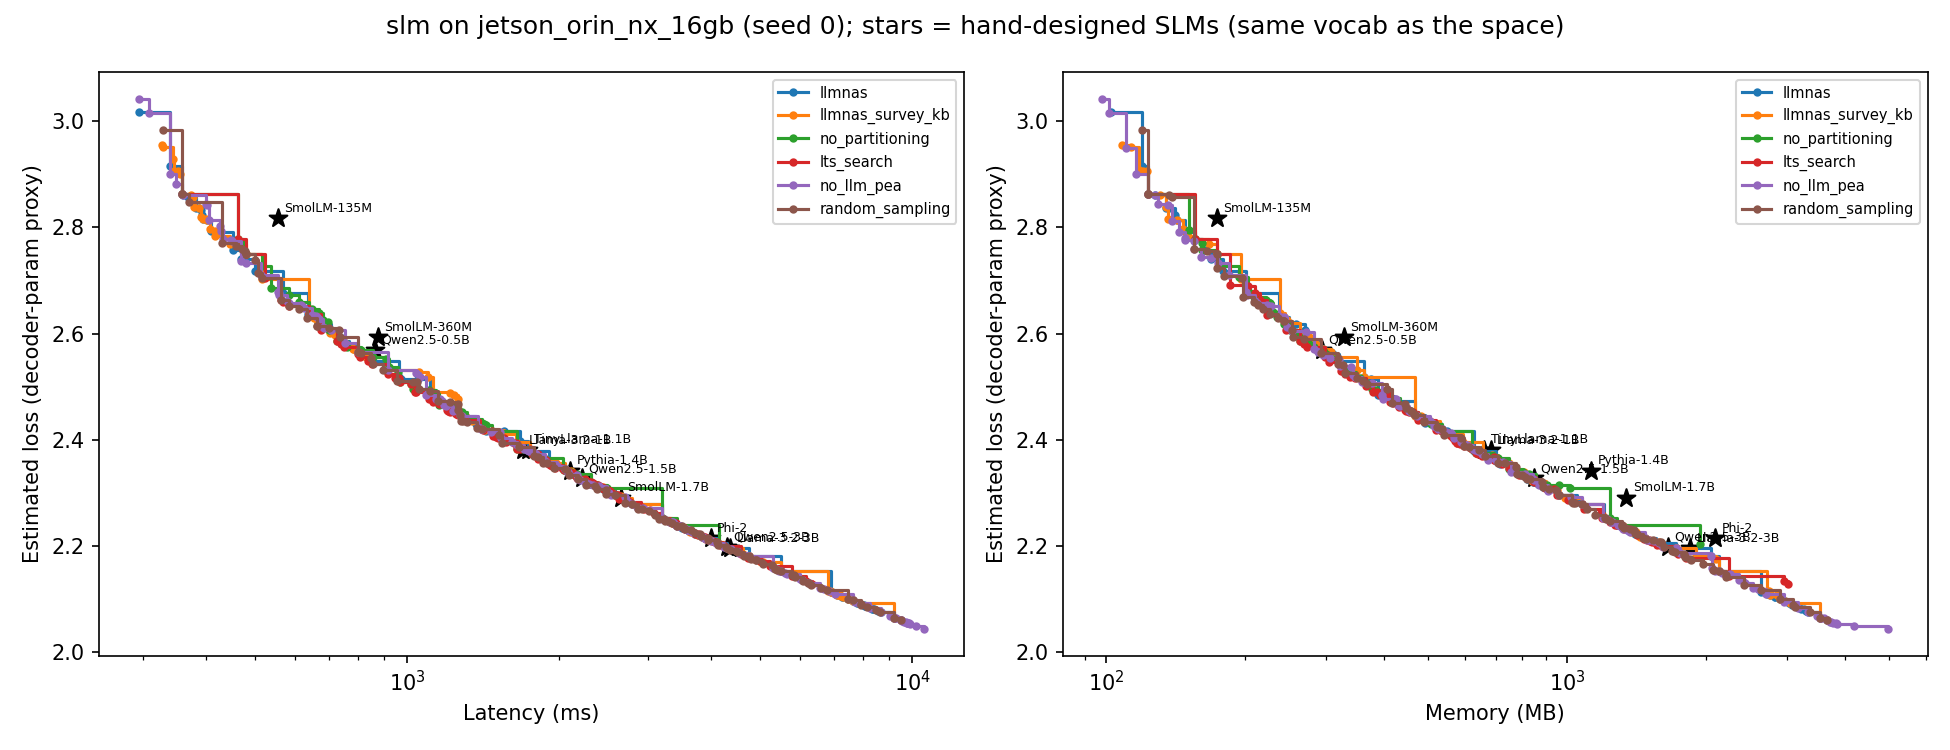
\includegraphics[width=\textwidth]{fronts_slm_jetson_orin_nx_16gb.png}
\caption{Fronts in the \code{slm} space on the Jetson cost model (seed 0). Stars are hand-designed SLMs evaluated with the same cost model and vocabulary.}\label{fig:slmfronts}
\end{figure}

\begin{figure}[h]\centering
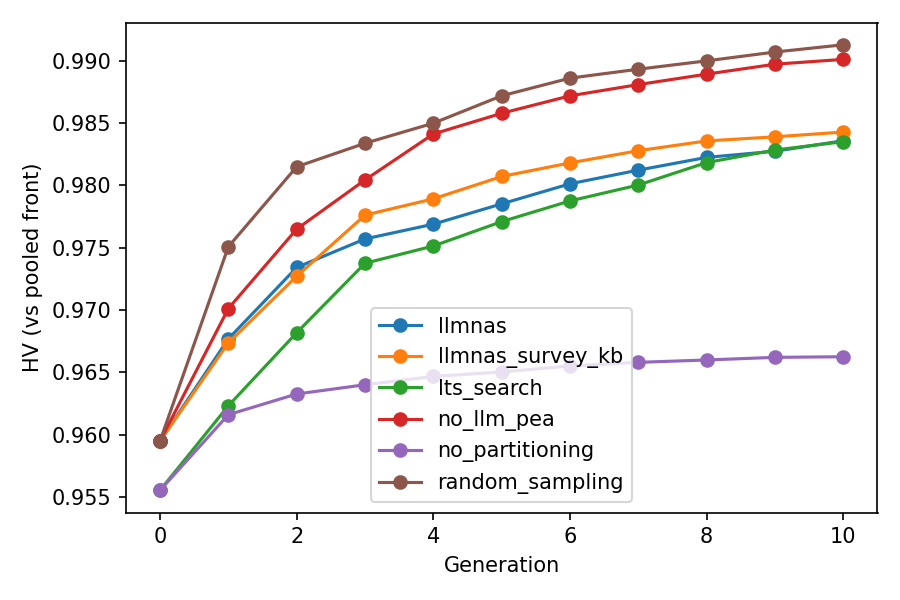
\includegraphics[width=0.6\textwidth]{slm_convergence.png}
\caption{HV against the pooled front per generation (mean over runs). The LLM variants start from the same 30 random samples and gain little thereafter.}\label{fig:slmconv}
\end{figure}

\paragraph{Comparison with hand-designed SLMs.} For each reference model we report the fastest searched architecture with at least as many decoder parameters (i.e.\ at least the same proxy quality), under the same cost model and vocabulary. On the Jetson model the searched shapes are $1.41\times$ faster than SmolLM-135M (393 vs.\ 555\,ms for a 50+50-token workload), $1.19\times$ faster than SmolLM-360M and $1.08\times$ faster than Qwen2.5-0.5B; from about 1B parameters upward the gain vanishes ($0.92$--$1.02\times$). On the Snapdragon model the corresponding figures are $1.20\times$, $1.02\times$ and $1.00\times$. The deep, narrow small models (SmolLM-135M has 30 layers of width 576) pay a per-layer overhead that the cost model, following the survey, charges in prefill; the larger SLMs are already close to the modelled optimum.

%=====================================================================
\section{Discussion: what was discovered}\label{sec:discussion}
\begin{enumerate}
  \item \textbf{The paper's data and encoding are recoverable, with two caveats.} Eleven of twelve Table-2 points are reproduced exactly; one (Edge GPU 94.37\% @ 4.35\,ms) does not exist in HW-NAS-Bench. The Edge TPU column of HW-NAS-Bench contains 4{,}699 placeholder values that must be excluded; this is not mentioned in the paper and materially changes Edge TPU numbers.
  \item \textbf{The HV convention is the dominant unknown.} Under the natural normalisation, 30 random samples already reach $\HV=0.88$ and random sampling within niches reaches $0.99$. The paper's reported gaps (full model 0.978 vs.\ PEA 0.843 on CIFAR-100) cannot be reproduced without a convention that penalises coverage gaps more heavily than ours. Until the authors specify their reference point and normalisation, HV comparisons across papers in this space are not meaningful.
  \item \textbf{Partitioning is the component that works.} In both domains, removing the niches is the worst configuration: on transformers it loses 10 percentage points of size coverage and doubles the latency overhead on Snapdragon. This is a genuine, transferable confirmation of the paper's exploration-bias argument.
  \item \textbf{The LLM operator did not beat random proposals inside the niches.} With Qwen2.5-7B this holds in both domains, with the LLM significantly worse than random sampling on transformers ($p=0.04$) and markedly noisier across seeds. With GPT-4.1 (one CNN seed) the LLM is better than Qwen but still below PEA and random sampling. The mechanism is visible in the proposal statistics: 50--60\% of LLM proposals are discarded as out-of-niche or duplicate, so the LLM evaluates roughly half as many new architectures as the baselines for the same budget.
  \item \textbf{Published prior knowledge did not help a 7B model.} Seeding the knowledge base with the survey's insights changed nothing measurable ($p=0.94$). Qwen also wrote incorrect rules from small samples (e.g.\ ``use $n_{\text{layer}}\ge9$ \ldots because it reduces latency''), which the co-evolution loop did not reliably correct.
  \item \textbf{Shape matters for small models under the survey's cost structure.} At matched decoder parameters the search found shapes 1.2--1.4$\times$ faster than the smallest published SLMs, while models above $\approx$1B are already near the modelled optimum. This is consistent with LTS's finding and gives a concrete, testable design recommendation (fewer, wider layers below 500M parameters).
  \item \textbf{A metric that reads as a claim.} Latency overhead at matched quality separates methods where HV cannot, decomposes by niche, and converts directly into statements such as ``method A's best 300M model is 5\% slower than the best known''. We recommend it, alongside coverage, for any benchmark where quality is a monotone proxy.
\end{enumerate}

\section{Threats to validity}
\begin{itemize}[nosep]
  \item \textbf{Single GPT-4.1 seed.} The paper's own LLM was run once, on one setting, because of budget; its 0.964 could move by $\pm0.03$ across seeds (the Qwen seed-to-seed spread on transformers was that large).
  \item \textbf{Local 7B model $\ne$ paper setting.} Qwen results are a reproduction with a substituted LLM and are reported as such.
  \item \textbf{Assumed hyper-parameters} (Table~\ref{tab:assumed}); the number of children per call and the predictor training size are plausible drivers of the remaining gap.
  \item \textbf{Stronger predictor than the paper's} (Spearman 0.96 vs.\ 0.90), which should help all methods equally but is a difference.
  \item \textbf{Cost model for the SLM extension.} Jetson and phone profiles are fitted by eye to the survey's figures; only the local CPU profile is calibrated against measurements. The quality proxy ignores training data and tokenizer, which the survey finds dominate; claims are therefore about architecture at a fixed training recipe.
  \item \textbf{Pooled-front HV} is comparable only within an experiment.
\end{itemize}

%=====================================================================
\section{Future work}\label{sec:future}
Ordered by cost and by how much each would change the conclusions:
\begin{enumerate}
  \item \textbf{Obtain the paper's HV/IGD convention from the authors} (reference point, normalisation, whether $S$ is the archive or all evaluated architectures) and re-score the archived runs with it. Zero cost; the replay logs make this a one-line change.
  \item \textbf{GPT-4.1 with three seeds on both domains} (CNN: 360 calls; SLM: 480 calls; $\approx\$5$--8 total at list price). This is the single experiment that decides whether finding~4 is a model-capability effect or a property of the method.
  \item \textbf{Fix the proposal-waste mechanism and re-test.} Three cheap interventions, each one config flag: (a) reject-and-retry out-of-niche proposals within the same call; (b) show the LLM the full evaluated set, not only parents, to reduce duplicates; (c) constrained decoding / JSON schema with the niche's counts enforced. If the LLM operator still trails random sampling once its usable rate matches the baselines', the negative result is robust.
  \item \textbf{Sensitivity study on the assumed hyper-parameters} (children per call $\in\{2,4,8\}$, predictor $n_{\text{train}}\in\{200,1000,5000\}$, parents shown), reported as HV and as latency overhead.
  \item \textbf{Exploration-bias study (paper's Figure~1/9).} The \code{fig1\_bias} experiment is implemented (normal vs.\ latency-optimised prompting) but has not been run; 10--20 calls per device.
  \item \textbf{Calibrate the SLM cost model on real devices.} Run \code{slm-calibrate} on the RTX~3050~Ti (CUDA PyTorch is available in the \code{hw-nas} environment) and, ideally, on a Jetson or Android phone with \code{llama.cpp} at Q4, then re-run \code{slm\_main} with measured latency in the loop.
  \item \textbf{Train a handful of front models} (as LTS trained 20) on a small corpus such as FineWeb-Edu to verify that the decoder-parameter proxy ranks the searched shapes correctly and that the 1.4$\times$ speed-up at matched quality survives real training.
  \item \textbf{Two-objective and constrained formulations.} Memory tracks parameter count almost exactly; treat memory as a constraint (\code{hardware.latency\_limit\_ms} and a memory cap) and search (quality, latency) only, which should sharpen all metrics.
  \item \textbf{Richer SLM spaces.} Add adaptive input embeddings (LTS), per-layer scaling (OpenELM), vocabulary size as a searchable variable with a quality penalty, and quantisation format as a hardware variable.
  \item \textbf{Alternative LLMs at fixed budget.} GPT-4.1-mini, Claude Sonnet~5.5 and a 14B local model would map the ``capability vs.\ benefit'' curve suggested by the GPT-4.1/Qwen gap.
  \item \textbf{Automate niche discovery} (the paper's own future-work item): cluster the search space by a cheap complexity statistic and compare learned niches with the hand-designed ones.
\end{enumerate}

\section{Reproducibility and artefacts}
All code, configurations, calibration files and reports are in the \code{llm-nas-repro} repository (nine commits, 44 passing tests). Benchmark data (2\,GB) is re-created by \code{python -m llmnas prepare-data}. The archived \code{results/runs/} directory (per run: \code{config.yaml}, \code{run.json}, \code{llm\_calls.jsonl}) is the evidence behind every number in this report; \code{python -m llmnas report <experiment>} regenerates all tables and figures, and \code{--set llm.mode=replay} re-executes any LLM search without API access. A Colab notebook performs the same steps with data and results on Google Drive.

%=====================================================================
\appendix
\section{Glossary of terms and formulas}\label{sec:glossary}
\begin{description}[style=nextline,leftmargin=0pt,itemsep=3pt]

\item[Architecture code (NB201).] A 6-tuple $(a,b,c,d,e,f)\in\{0,\dots,4\}^6$ giving the operator on each edge of the 4-node cell in the order $n_1{\leftarrow}n_0,\ n_2{\leftarrow}n_0,\ n_2{\leftarrow}n_1,\ n_3{\leftarrow}n_0,\ n_3{\leftarrow}n_1,\ n_3{\leftarrow}n_2$, with $0$=\code{none}, $1$=\code{skip\_connect}, $2$=\code{nor\_conv\_1x1}, $3$=\code{nor\_conv\_3x3}, $4$=\code{avg\_pool\_3x3}.

\item[Calibration (cost model).] Least-squares fit of $t = a\cdot w + b\cdot n_{\text{layer}} + c$ separately for prefill ($w$ = FLOPs) and decode ($w$ = bytes per token) to measured times; quality reported as Spearman correlation and mean absolute percentage error between modelled and measured latency.

\item[Configuration hash.] SHA-1 (first 8 hex digits) of the canonical JSON of a run's effective configuration, excluding fields that cannot affect results. Identical settings map to the same run directory.

\item[Coverage.] Fraction of the $K$ decoder-parameter levels $N_k$ at which a run has at least one feasible model with $\ge N_k$ decoder parameters.

\item[Crossover / mutation.] Evolutionary operators. Uniform crossover copies each gene from parent $A$ or $B$ with probability $\tfrac12$; mutation re-draws one gene (NB201) or each gene with probability $p=0.3$ (LTS).

\item[Decoder parameters.] Non-embedding parameters of a decoder-only transformer. Per layer with model width $d$, head dimension $h=d/n_{\text{head}}$, $n_{\text{kv}}$ key/value heads and FFN width $d_{\text{inner}}$:
\[
P_{\text{layer}} = \underbrace{2d^2 + 2\,d\,n_{\text{kv}}\,h}_{\text{attention }(q,o;\,k,v)} + \underbrace{m\,d\,d_{\text{inner}}}_{\text{FFN}} + 2d,\qquad m=\begin{cases}3 & \text{gated (SwiGLU)}\\ 2 & \text{standard}\end{cases}
\]
and $P_{\text{dec}}=\sum_{\text{layers}}P_{\text{layer}}+d$. Total parameters add $V\!\cdot\! d$ (tied embeddings) or $2V\!\cdot\! d$ (untied), $V$ = vocabulary size. LTS's zero-cost quality proxy.

\item[Exploration bias / mode collapse.] The tendency of a generative model to repeatedly propose a narrow family of outputs. LLM-NAS's motivation for niching.

\item[FLOPs (prefill).] For a prompt of $P$ tokens: $\text{FLOPs}\approx 2P\,P_{\text{dec}} + \sum_{\text{layers}}2P^2 d + 2dV$ (dense matmuls, causal attention, final logits).

\item[Grouped-query attention (GQA) / MQA / MHA.] Attention with $n_{\text{kv}}$ key/value heads shared among $n_{\text{head}}$ query heads; $n_{\text{kv}}=n_{\text{head}}$ is multi-head (MHA), $n_{\text{kv}}=1$ is multi-query (MQA). KV-cache bytes per token scale with $n_{\text{kv}}$.

\item[Hypervolume (HV).] For a set $S$ of points in $m$-objective space (minimisation) and a reference point $r$ dominated by all of $S$,
\[
\HV(S,r)=\lambda\Big(\bigcup_{s\in S}[s_1,r_1]\times\cdots\times[s_m,r_m]\Big),
\]
the Lebesgue measure of the dominated region. We report the ratio $\HV(S,r)/\HV(P^\ast,r)$ after min--max normalising each objective by the ideal and nadir points of the true front $P^\ast$, with $r=(1.1,\dots,1.1)$. In 2-D it is computed by sorting the front and summing rectangles; in 3-D by slicing along the third objective.

\item[Inverted generational distance (IGD).]
\[
\IGD(S,P^\ast)=\frac{1}{|P^\ast|}\sum_{p\in P^\ast}\min_{s\in S}\lVert p-s\rVert_2,
\]
the mean distance from each true-front point to its nearest discovered point (normalised objectives). Lower is better; zero iff $S\supseteq P^\ast$.

\item[Isotonic regression.] Monotone non-decreasing least-squares fit; used to map Synflow scores to the accuracy scale without changing their ranking.

\item[Kaplan scaling law.] $L(N)=(N_c/N)^{\alpha_N}$ with $N_c=8.8\times10^{13}$, $\alpha_N=0.076$: the estimated language-model loss as a function of non-embedding parameters $N$. Monotone in $N$, so it ranks exactly as the decoder-parameter proxy; used only to give the LLM an interpretable number.

\item[Knowledge base (co-evolve).] A list of natural-language rules of the form ``use/avoid \ldots because \ldots'' that the LLM rewrites after each generation from the previous cycle's results and that is injected into the next generation prompt.

\item[KV cache.] Stored keys and values for past tokens: bytes $=\sum_{\text{layers}}2\,n_{\text{kv}}\,h\,T\,b$ for $T$ tokens at $b$ bytes per element (2 for fp16).

\item[Latency overhead at matched quality.] With levels $N_1<\dots<N_K$ (log-spaced over the pooled front), $t^\ast(N_k)=\min\{\text{latency}(x): P_{\text{dec}}(x)\ge N_k,\ x\in\text{any run}\}$ and $t_m(N_k)$ the same restricted to run $m$,
\[
\text{Overhead}_m=\exp\!\Big(\frac{1}{|K_m|}\sum_{k\in K_m}\ln\frac{t_m(N_k)}{t^\ast(N_k)}\Big)-1,\qquad K_m=\{k: t_m(N_k)\text{ exists}\},
\]
a geometric-mean slowdown relative to the best known model of at least the same proxy quality. Zero means the run is best everywhere it reaches.

\item[Mann--Whitney $U$ test.] Non-parametric two-sample test of whether one distribution is stochastically larger than another; used here with $n=6$ runs per variant, two-sided.

\item[Min--max normalisation.] $\tilde{x}_j=(x_j-\min_j)/(\max_j-\min_j)$ per objective $j$, with min/max taken over the true front (or the pooled front) so that normalised objectives lie in $[0,1]$ on the front.

\item[NAS-Bench-201 / NATS-Bench / HW-NAS-Bench / NAS-Bench-Suite-Zero.] Tabular benchmarks: NB201 (= NATS-Bench topology space) gives trained accuracy for all 15{,}625 cells on CIFAR-10/100 and ImageNet16-120; HW-NAS-Bench adds measured latency/energy on six devices; NAS-Bench-Suite-Zero adds 13 zero-cost proxy scores per architecture.

\item[Niche (partitioning).] A disjoint subset of the search space defined by a complexity statistic: number of $3{\times}3$ convolutions (CNN, Table~1 of LLM-NAS) or a band of decoder parameters (SLM). Each niche keeps its own Pareto archive; archives are merged by non-dominated sorting at the end.

\item[Pareto dominance / front.] For minimisation, $a\preceq b$ iff $a_j\le b_j\ \forall j$ and $a_j<b_j$ for some $j$. The Pareto front is the set of non-dominated points. The \emph{pooled reference front} is the front of all feasible points evaluated by any run of an experiment.

\item[PEA (partitioned evolutionary algorithm).] LLM-NAS's ``without LLM operator'' ablation: the same niches, archives and budget, with random mutation/crossover in place of the LLM.

\item[Prefill / decode.] The two phases of autoregressive inference: processing the prompt in parallel (compute-bound; time $\approx$ FLOPs / effective throughput) and generating one token at a time (memory-bound; time $\approx$ bytes read per token / effective bandwidth). End-to-end latency for the survey's workload $= t_{\text{prefill}}(50)+50\,t_{\text{decode}}$.

\item[Quantisation (Q4\_K\_M).] 4-bit weight storage in \code{llama.cpp}'s k-quant format, $\approx0.56$ bytes per parameter; the survey's best-performing setting and our default for modelled memory and decode bytes.

\item[Replay.] Re-execution of a search with LLM responses taken from the saved call log instead of the API; must reproduce the original run exactly (mismatch counter 0).

\item[Roofline model.] Time $=\max(\text{compute}/\text{peak throughput},\ \text{bytes}/\text{bandwidth})$ scaled by an efficiency factor; the basis of the analytical prefill estimate.

\item[Seed.] Integer fixing a run's pseudo-random choices (initial population, predictor training sample, parent selection, crossover/mutation assignment, and the LLM sampling hint). Different seeds give independent repeats; results are reported as mean $\pm$ standard deviation over seeds.

\item[Spearman / Kendall rank correlation.] $\rho=1-\frac{6\sum d_i^2}{n(n^2-1)}$ over rank differences $d_i$ (Spearman); $\tau=\frac{C-D}{\binom{n}{2}}$ over concordant/discordant pairs (Kendall). Used to validate predictors and cost models against ground truth.

\item[SwiGLU / gated FFN.] Feed-forward block $W_2\,(\mathrm{SiLU}(W_1x)\odot W_3x)$ with three weight matrices (vs.\ two in the standard $W_2\,\sigma(W_1x)$ block); the dominant choice in 2024 SLMs.

\item[Usable proposal rate.] Fraction of LLM (or operator) proposals that parse, satisfy the niche constraint and are not duplicates of already-evaluated architectures; the remainder consume budget without an evaluation.

\item[XGBoost.] Gradient-boosted decision-tree regressor; here with 500 trees of depth 6, learning rate 0.05, trained on the 13 ZC proxies.

\item[Zero-cost (ZC) proxy.] A score computed from an untrained network (one forward/backward pass or less) that correlates with trained accuracy, e.g.\ \code{synflow}, \code{snip}, \code{grasp}, \code{fisher}, \code{jacov}, \code{nwot}, \code{zen}, \code{epe\_nas}, \code{grad\_norm}, \code{l2\_norm}, \code{plain}, \code{params}, \code{flops}.
\end{description}

\begin{thebibliography}{9}
\bibitem{llmnas} H.~Zhu, G.~L.~Zhang, S.~Huang. LLM-NAS: LLM-Driven Hardware-Aware Neural Architecture Search. \emph{arXiv:2510.01472v4}, 2025.
\bibitem{lts} M.~Javaheripi et al. LiteTransformerSearch: Training-free Neural Architecture Search for Efficient Language Models. \emph{NeurIPS}, 2022. arXiv:2203.02094.
\bibitem{slmsurvey} Z.~Lu, X.~Li, D.~Cai, R.~Yi, F.~Liu, X.~Zhang, N.~D.~Lane, M.~Xu. Small Language Models: Survey, Measurements, and Insights. \emph{arXiv:2409.15790v3}, 2025.
\bibitem{hwnasbench} C.~Li et al. HW-NAS-Bench: Hardware-Aware Neural Architecture Search Benchmark. \emph{ICLR}, 2021.
\bibitem{nbsz} A.~Krishnakumar, C.~White, A.~Zela, R.~Tu, M.~Safari, F.~Hutter. NAS-Bench-Suite-Zero: Accelerating Research on Zero Cost Proxies. \emph{NeurIPS Datasets and Benchmarks}, 2022.
\bibitem{nats} X.~Dong, L.~Liu, K.~Musial, B.~Gabrys. NATS-Bench: Benchmarking NAS Algorithms for Architecture Topology and Size. \emph{IEEE TPAMI}, 2021.
\bibitem{kaplan} J.~Kaplan et al. Scaling Laws for Neural Language Models. \emph{arXiv:2001.08361}, 2020.
\end{thebibliography}

\end{document}
